\documentclass[../rapport_MVEX01-11-05]{subfiles}
\begin{document}

\subsection{Egenskaper}\label{sec:resultat_features}

Egenskaper kan förstås variera i kvalitet och det är därför viktigt att
verifiera att de egenskaper som används verkligen gör det möjligt för
klassificeringsalgoritmen att skilja på olika gester. Detta innebär att en
gest inte kan variera mycket inom en gest --- för en enskild gest ska 
egenskapen alltså endast anta värden på ett delintervall till värdemängden ---
och att en egenskap gärna även ska variera mycket mellan gester, dvs.~att
delintervallen inte överlappar.

Det är alltså viktigt för \knn-metoden att
egenskapsrummet är utformat så att bilder från varje gest är både tydligt
separerade och tydligt grupperade. Det viktigaste är grupperingen; att gester
är separerade är något som endast förenklar processen.
Trots att gesterna ligger mycket tätt i vårt egenskapsrum så är de redan i det
tvådimensionella underrummet till egenskapsrummet som visas i figur~\ref{fig:feats1011}
mycket tydligt grupperade, vilket gör att \knn-metoden ger exakta resultat.

\begin{figure}[tb]
  \centering
  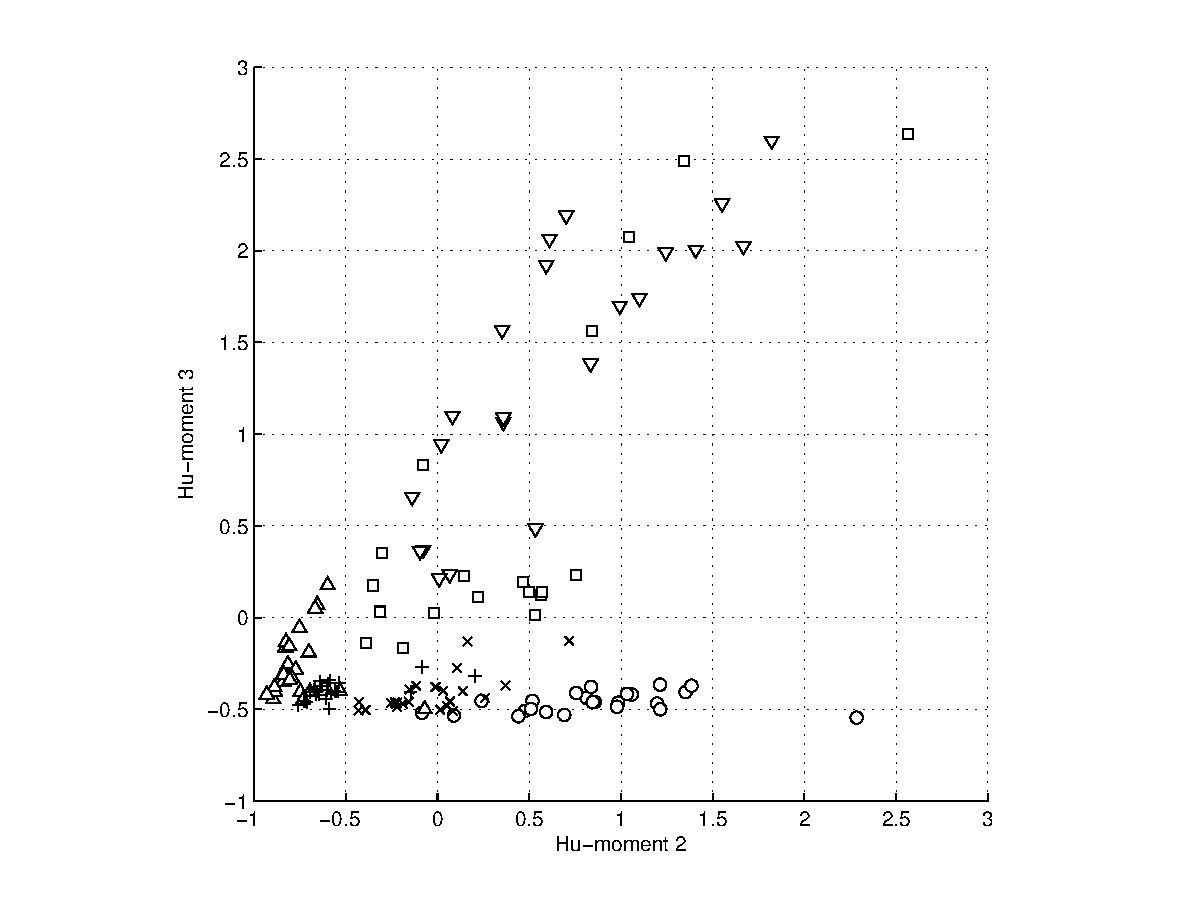
\includegraphics[width=\textwidth,trim=2cm 0.5cm 2cm 0]{bilder/feats-10+11}
  \caption{De två starkaste egenskaperna för prototypdatan}
  \label{fig:feats1011}
\end{figure}

Fler egenskaper än de två i figur~\ref{fig:feats1011} ger inte helt oväntat
(men inte heller trivialt) ett bättre resultat. Figur~\ref{fig:knn-optimering} visar
hur det relativa felet minskar både då $k$ ökar i \knn-metoden och då antalet
egenskaper som inkluderas i rummet ökar. Något mer oväntat är dock att det
finns ett tydligt minimum som inte inkluderar alla egenskaper.

Det är även intressant att veta vilka av egenskaperna som är ''bäst'' när det
gäller att klassificera gester. Tabell~\ref{tab:bestfeats} listar de tio bästa
egenskaperna i den ordning \notes{vårt skript? sorterar dem?}

\begin{table}[tb]
	\centering
	\caption{De tio bästa egenskaperna}
	\label{tab:bestfeats}
	\begin{tabular}{ll}
		\toprule
		Ranking & Gest \\
		\midrule
		1 & Hu-moment 3 \\
		2 & Hu-moment 2 \\
		3 & Centroidläge, Y-led \\
		4 & Fyrkantighet \\
		5 & Soliditet \\
		6 & Excentricitet \\
		7 & Konvexitet \\
		8 & Hu-moment 1 \\
		9 & Utsträckning \\
		10 & Hu-moment 7 \\
		\bottomrule
	\end{tabular}
\end{table}

\end{document}